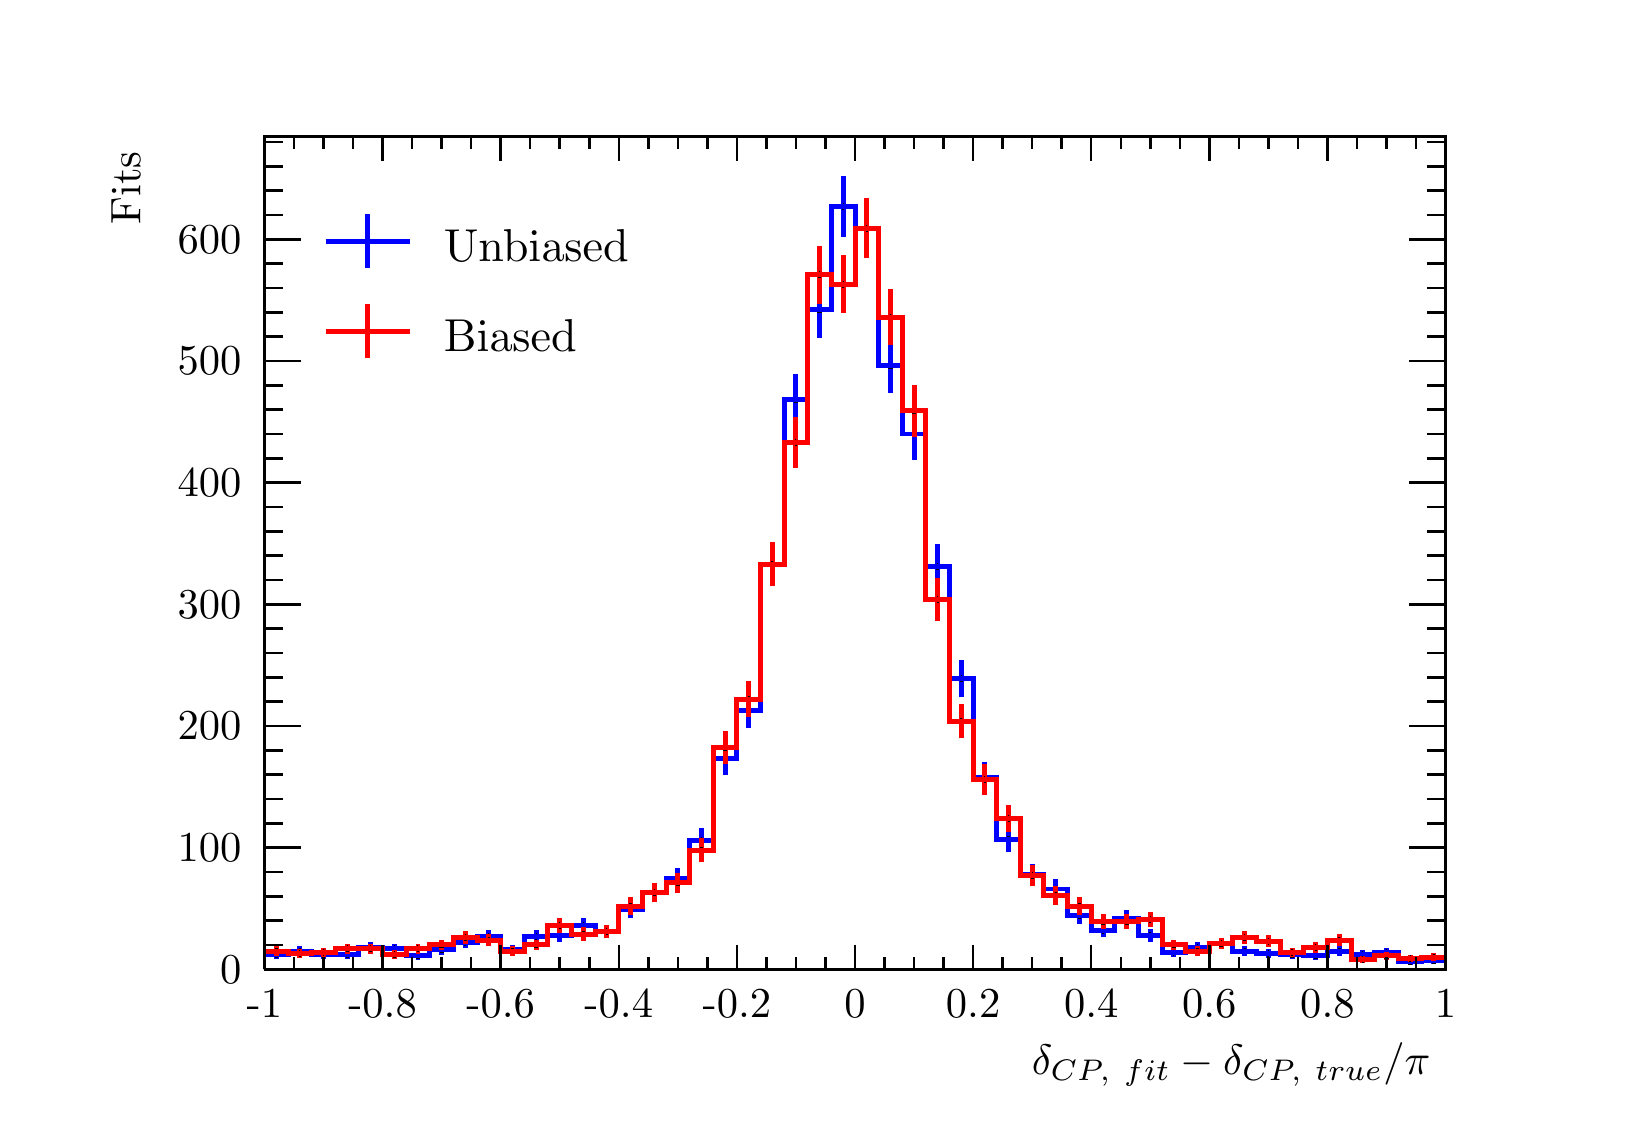
\begin{tikzpicture}
\pgfdeclareplotmark{cross} {
\pgfpathmoveto{\pgfpoint{-0.3\pgfplotmarksize}{\pgfplotmarksize}}
\pgfpathlineto{\pgfpoint{+0.3\pgfplotmarksize}{\pgfplotmarksize}}
\pgfpathlineto{\pgfpoint{+0.3\pgfplotmarksize}{0.3\pgfplotmarksize}}
\pgfpathlineto{\pgfpoint{+1\pgfplotmarksize}{0.3\pgfplotmarksize}}
\pgfpathlineto{\pgfpoint{+1\pgfplotmarksize}{-0.3\pgfplotmarksize}}
\pgfpathlineto{\pgfpoint{+0.3\pgfplotmarksize}{-0.3\pgfplotmarksize}}
\pgfpathlineto{\pgfpoint{+0.3\pgfplotmarksize}{-1.\pgfplotmarksize}}
\pgfpathlineto{\pgfpoint{-0.3\pgfplotmarksize}{-1.\pgfplotmarksize}}
\pgfpathlineto{\pgfpoint{-0.3\pgfplotmarksize}{-0.3\pgfplotmarksize}}
\pgfpathlineto{\pgfpoint{-1.\pgfplotmarksize}{-0.3\pgfplotmarksize}}
\pgfpathlineto{\pgfpoint{-1.\pgfplotmarksize}{0.3\pgfplotmarksize}}
\pgfpathlineto{\pgfpoint{-0.3\pgfplotmarksize}{0.3\pgfplotmarksize}}
\pgfpathclose
\pgfusepathqstroke
}
\pgfdeclareplotmark{cross*} {
\pgfpathmoveto{\pgfpoint{-0.3\pgfplotmarksize}{\pgfplotmarksize}}
\pgfpathlineto{\pgfpoint{+0.3\pgfplotmarksize}{\pgfplotmarksize}}
\pgfpathlineto{\pgfpoint{+0.3\pgfplotmarksize}{0.3\pgfplotmarksize}}
\pgfpathlineto{\pgfpoint{+1\pgfplotmarksize}{0.3\pgfplotmarksize}}
\pgfpathlineto{\pgfpoint{+1\pgfplotmarksize}{-0.3\pgfplotmarksize}}
\pgfpathlineto{\pgfpoint{+0.3\pgfplotmarksize}{-0.3\pgfplotmarksize}}
\pgfpathlineto{\pgfpoint{+0.3\pgfplotmarksize}{-1.\pgfplotmarksize}}
\pgfpathlineto{\pgfpoint{-0.3\pgfplotmarksize}{-1.\pgfplotmarksize}}
\pgfpathlineto{\pgfpoint{-0.3\pgfplotmarksize}{-0.3\pgfplotmarksize}}
\pgfpathlineto{\pgfpoint{-1.\pgfplotmarksize}{-0.3\pgfplotmarksize}}
\pgfpathlineto{\pgfpoint{-1.\pgfplotmarksize}{0.3\pgfplotmarksize}}
\pgfpathlineto{\pgfpoint{-0.3\pgfplotmarksize}{0.3\pgfplotmarksize}}
\pgfpathclose
\pgfusepathqfillstroke
}
\pgfdeclareplotmark{newstar} {
\pgfpathmoveto{\pgfqpoint{0pt}{\pgfplotmarksize}}
\pgfpathlineto{\pgfqpointpolar{44}{0.5\pgfplotmarksize}}
\pgfpathlineto{\pgfqpointpolar{18}{\pgfplotmarksize}}
\pgfpathlineto{\pgfqpointpolar{-20}{0.5\pgfplotmarksize}}
\pgfpathlineto{\pgfqpointpolar{-54}{\pgfplotmarksize}}
\pgfpathlineto{\pgfqpointpolar{-90}{0.5\pgfplotmarksize}}
\pgfpathlineto{\pgfqpointpolar{234}{\pgfplotmarksize}}
\pgfpathlineto{\pgfqpointpolar{198}{0.5\pgfplotmarksize}}
\pgfpathlineto{\pgfqpointpolar{162}{\pgfplotmarksize}}
\pgfpathlineto{\pgfqpointpolar{134}{0.5\pgfplotmarksize}}
\pgfpathclose
\pgfusepathqstroke
}
\pgfdeclareplotmark{newstar*} {
\pgfpathmoveto{\pgfqpoint{0pt}{\pgfplotmarksize}}
\pgfpathlineto{\pgfqpointpolar{44}{0.5\pgfplotmarksize}}
\pgfpathlineto{\pgfqpointpolar{18}{\pgfplotmarksize}}
\pgfpathlineto{\pgfqpointpolar{-20}{0.5\pgfplotmarksize}}
\pgfpathlineto{\pgfqpointpolar{-54}{\pgfplotmarksize}}
\pgfpathlineto{\pgfqpointpolar{-90}{0.5\pgfplotmarksize}}
\pgfpathlineto{\pgfqpointpolar{234}{\pgfplotmarksize}}
\pgfpathlineto{\pgfqpointpolar{198}{0.5\pgfplotmarksize}}
\pgfpathlineto{\pgfqpointpolar{162}{\pgfplotmarksize}}
\pgfpathlineto{\pgfqpointpolar{134}{0.5\pgfplotmarksize}}
\pgfpathclose
\pgfusepathqfillstroke
}
\definecolor{c}{rgb}{1,1,1};
\draw [color=c, fill=c] (0,0) rectangle (20,13.7374);
\draw [color=c, fill=c] (3,1.78586) rectangle (18,12.3636);
\definecolor{c}{rgb}{0,0,0};
\draw [c,line width=0.9] (3,1.78586) -- (3,12.3636) -- (18,12.3636) -- (18,1.78586) -- (3,1.78586);
\definecolor{c}{rgb}{1,1,1};
\draw [color=c, fill=c] (3,1.78586) rectangle (18,12.3636);
\definecolor{c}{rgb}{0,0,0};
\draw [c,line width=0.9] (3,1.78586) -- (3,12.3636) -- (18,12.3636) -- (18,1.78586) -- (3,1.78586);
\draw [c,line width=0.9] (3,1.78586) -- (3.3,1.78586) -- (3.3,1.78586) -- (3.6,1.78586) -- (3.6,1.78586) -- (3.9,1.78586) -- (3.9,1.78586) -- (4.2,1.78586) -- (4.2,1.78586) -- (4.5,1.78586) -- (4.5,1.78586) -- (4.8,1.78586) -- (4.8,1.78586) --
 (5.1,1.78586) -- (5.1,1.78586) -- (5.4,1.78586) -- (5.4,1.78586) -- (5.7,1.78586) -- (5.7,1.78586) -- (6,1.78586) -- (6,1.78586) -- (6.3,1.78586) -- (6.3,1.78586) -- (6.6,1.78586) -- (6.6,1.78586) -- (6.9,1.78586) -- (6.9,1.78586) -- (7.2,1.78586)
 -- (7.2,1.78586) -- (7.5,1.78586) -- (7.5,1.78586) -- (7.8,1.78586) -- (7.8,1.78586) -- (8.1,1.78586) -- (8.1,1.78586) -- (8.4,1.78586) -- (8.4,1.78586) -- (8.7,1.78586) -- (8.7,1.78586) -- (9,1.78586) -- (9,1.78586) -- (9.3,1.78586) --
 (9.3,1.78586) -- (9.6,1.78586) -- (9.6,1.78586) -- (9.9,1.78586) -- (9.9,1.78586) -- (10.2,1.78586) -- (10.2,1.78586) -- (10.5,1.78586) -- (10.5,1.78586) -- (10.8,1.78586) -- (10.8,1.78586) -- (11.1,1.78586) -- (11.1,1.78586) -- (11.4,1.78586) --
 (11.4,1.78586) -- (11.7,1.78586) -- (11.7,1.78586) -- (12,1.78586) -- (12,1.78586) -- (12.3,1.78586) -- (12.3,1.78586) -- (12.6,1.78586) -- (12.6,1.78586) -- (12.9,1.78586) -- (12.9,1.78586) -- (13.2,1.78586) -- (13.2,1.78586) -- (13.5,1.78586) --
 (13.5,1.78586) -- (13.8,1.78586) -- (13.8,1.78586) -- (14.1,1.78586) -- (14.1,1.78586) -- (14.4,1.78586) -- (14.4,1.78586) -- (14.7,1.78586) -- (14.7,1.78586) -- (15,1.78586) -- (15,1.78586) -- (15.3,1.78586) -- (15.3,1.78586) -- (15.6,1.78586) --
 (15.6,1.78586) -- (15.9,1.78586) -- (15.9,1.78586) -- (16.2,1.78586) -- (16.2,1.78586) -- (16.5,1.78586) -- (16.5,1.78586) -- (16.8,1.78586) -- (16.8,1.78586) -- (17.1,1.78586) -- (17.1,1.78586) -- (17.4,1.78586) -- (17.4,1.78586) -- (17.7,1.78586)
 -- (17.7,1.78586) -- (18,1.78586);
\draw [c,line width=0.9] (3,1.78586) -- (18,1.78586);
\draw [c,line width=0.9] (3,2.09495) -- (3,1.78586);
\draw [c,line width=0.9] (3.375,1.9404) -- (3.375,1.78586);
\draw [c,line width=0.9] (3.75,1.9404) -- (3.75,1.78586);
\draw [c,line width=0.9] (4.125,1.9404) -- (4.125,1.78586);
\draw [c,line width=0.9] (4.5,2.09495) -- (4.5,1.78586);
\draw [c,line width=0.9] (4.875,1.9404) -- (4.875,1.78586);
\draw [c,line width=0.9] (5.25,1.9404) -- (5.25,1.78586);
\draw [c,line width=0.9] (5.625,1.9404) -- (5.625,1.78586);
\draw [c,line width=0.9] (6,2.09495) -- (6,1.78586);
\draw [c,line width=0.9] (6.375,1.9404) -- (6.375,1.78586);
\draw [c,line width=0.9] (6.75,1.9404) -- (6.75,1.78586);
\draw [c,line width=0.9] (7.125,1.9404) -- (7.125,1.78586);
\draw [c,line width=0.9] (7.5,2.09495) -- (7.5,1.78586);
\draw [c,line width=0.9] (7.875,1.9404) -- (7.875,1.78586);
\draw [c,line width=0.9] (8.25,1.9404) -- (8.25,1.78586);
\draw [c,line width=0.9] (8.625,1.9404) -- (8.625,1.78586);
\draw [c,line width=0.9] (9,2.09495) -- (9,1.78586);
\draw [c,line width=0.9] (9.375,1.9404) -- (9.375,1.78586);
\draw [c,line width=0.9] (9.75,1.9404) -- (9.75,1.78586);
\draw [c,line width=0.9] (10.125,1.9404) -- (10.125,1.78586);
\draw [c,line width=0.9] (10.5,2.09495) -- (10.5,1.78586);
\draw [c,line width=0.9] (10.875,1.9404) -- (10.875,1.78586);
\draw [c,line width=0.9] (11.25,1.9404) -- (11.25,1.78586);
\draw [c,line width=0.9] (11.625,1.9404) -- (11.625,1.78586);
\draw [c,line width=0.9] (12,2.09495) -- (12,1.78586);
\draw [c,line width=0.9] (12.375,1.9404) -- (12.375,1.78586);
\draw [c,line width=0.9] (12.75,1.9404) -- (12.75,1.78586);
\draw [c,line width=0.9] (13.125,1.9404) -- (13.125,1.78586);
\draw [c,line width=0.9] (13.5,2.09495) -- (13.5,1.78586);
\draw [c,line width=0.9] (13.875,1.9404) -- (13.875,1.78586);
\draw [c,line width=0.9] (14.25,1.9404) -- (14.25,1.78586);
\draw [c,line width=0.9] (14.625,1.9404) -- (14.625,1.78586);
\draw [c,line width=0.9] (15,2.09495) -- (15,1.78586);
\draw [c,line width=0.9] (15.375,1.9404) -- (15.375,1.78586);
\draw [c,line width=0.9] (15.75,1.9404) -- (15.75,1.78586);
\draw [c,line width=0.9] (16.125,1.9404) -- (16.125,1.78586);
\draw [c,line width=0.9] (16.5,2.09495) -- (16.5,1.78586);
\draw [c,line width=0.9] (16.875,1.9404) -- (16.875,1.78586);
\draw [c,line width=0.9] (17.25,1.9404) -- (17.25,1.78586);
\draw [c,line width=0.9] (17.625,1.9404) -- (17.625,1.78586);
\draw [c,line width=0.9] (18,2.09495) -- (18,1.78586);
\draw [c,line width=0.9] (3,2.09495) -- (3,1.78586);
\draw [anchor=base] (3,1.16768) node[scale=1.53833, color=c, rotate=0]{-1};
\draw [anchor=base] (4.5,1.16768) node[scale=1.53833, color=c, rotate=0]{-0.8};
\draw [anchor=base] (6,1.16768) node[scale=1.53833, color=c, rotate=0]{-0.6};
\draw [anchor=base] (7.5,1.16768) node[scale=1.53833, color=c, rotate=0]{-0.4};
\draw [anchor=base] (9,1.16768) node[scale=1.53833, color=c, rotate=0]{-0.2};
\draw [anchor=base] (10.5,1.16768) node[scale=1.53833, color=c, rotate=0]{0};
\draw [anchor=base] (12,1.16768) node[scale=1.53833, color=c, rotate=0]{0.2};
\draw [anchor=base] (13.5,1.16768) node[scale=1.53833, color=c, rotate=0]{0.4};
\draw [anchor=base] (15,1.16768) node[scale=1.53833, color=c, rotate=0]{0.6};
\draw [anchor=base] (16.5,1.16768) node[scale=1.53833, color=c, rotate=0]{0.8};
\draw [anchor=base] (18,1.16768) node[scale=1.53833, color=c, rotate=0]{1};
\draw [anchor= east] (18,0.57697) node[scale=1.53833, color=c, rotate=0]{$\delta_{CP,~\text{fit}} - \delta_{CP,~\text{true}} / \pi$};
\draw [c,line width=0.9] (3,12.3636) -- (18,12.3636);
\draw [c,line width=0.9] (3,12.0545) -- (3,12.3636);
\draw [c,line width=0.9] (3.375,12.2091) -- (3.375,12.3636);
\draw [c,line width=0.9] (3.75,12.2091) -- (3.75,12.3636);
\draw [c,line width=0.9] (4.125,12.2091) -- (4.125,12.3636);
\draw [c,line width=0.9] (4.5,12.0545) -- (4.5,12.3636);
\draw [c,line width=0.9] (4.875,12.2091) -- (4.875,12.3636);
\draw [c,line width=0.9] (5.25,12.2091) -- (5.25,12.3636);
\draw [c,line width=0.9] (5.625,12.2091) -- (5.625,12.3636);
\draw [c,line width=0.9] (6,12.0545) -- (6,12.3636);
\draw [c,line width=0.9] (6.375,12.2091) -- (6.375,12.3636);
\draw [c,line width=0.9] (6.75,12.2091) -- (6.75,12.3636);
\draw [c,line width=0.9] (7.125,12.2091) -- (7.125,12.3636);
\draw [c,line width=0.9] (7.5,12.0545) -- (7.5,12.3636);
\draw [c,line width=0.9] (7.875,12.2091) -- (7.875,12.3636);
\draw [c,line width=0.9] (8.25,12.2091) -- (8.25,12.3636);
\draw [c,line width=0.9] (8.625,12.2091) -- (8.625,12.3636);
\draw [c,line width=0.9] (9,12.0545) -- (9,12.3636);
\draw [c,line width=0.9] (9.375,12.2091) -- (9.375,12.3636);
\draw [c,line width=0.9] (9.75,12.2091) -- (9.75,12.3636);
\draw [c,line width=0.9] (10.125,12.2091) -- (10.125,12.3636);
\draw [c,line width=0.9] (10.5,12.0545) -- (10.5,12.3636);
\draw [c,line width=0.9] (10.875,12.2091) -- (10.875,12.3636);
\draw [c,line width=0.9] (11.25,12.2091) -- (11.25,12.3636);
\draw [c,line width=0.9] (11.625,12.2091) -- (11.625,12.3636);
\draw [c,line width=0.9] (12,12.0545) -- (12,12.3636);
\draw [c,line width=0.9] (12.375,12.2091) -- (12.375,12.3636);
\draw [c,line width=0.9] (12.75,12.2091) -- (12.75,12.3636);
\draw [c,line width=0.9] (13.125,12.2091) -- (13.125,12.3636);
\draw [c,line width=0.9] (13.5,12.0545) -- (13.5,12.3636);
\draw [c,line width=0.9] (13.875,12.2091) -- (13.875,12.3636);
\draw [c,line width=0.9] (14.25,12.2091) -- (14.25,12.3636);
\draw [c,line width=0.9] (14.625,12.2091) -- (14.625,12.3636);
\draw [c,line width=0.9] (15,12.0545) -- (15,12.3636);
\draw [c,line width=0.9] (15.375,12.2091) -- (15.375,12.3636);
\draw [c,line width=0.9] (15.75,12.2091) -- (15.75,12.3636);
\draw [c,line width=0.9] (16.125,12.2091) -- (16.125,12.3636);
\draw [c,line width=0.9] (16.5,12.0545) -- (16.5,12.3636);
\draw [c,line width=0.9] (16.875,12.2091) -- (16.875,12.3636);
\draw [c,line width=0.9] (17.25,12.2091) -- (17.25,12.3636);
\draw [c,line width=0.9] (17.625,12.2091) -- (17.625,12.3636);
\draw [c,line width=0.9] (18,12.0545) -- (18,12.3636);
\draw [c,line width=0.9] (3,12.0545) -- (3,12.3636);
\draw [c,line width=0.9] (3,1.78586) -- (3,12.3636);
\draw [c,line width=0.9] (3.462,1.78586) -- (3,1.78586);
\draw [c,line width=0.9] (3.231,2.09486) -- (3,2.09486);
\draw [c,line width=0.9] (3.231,2.40386) -- (3,2.40386);
\draw [c,line width=0.9] (3.231,2.71286) -- (3,2.71286);
\draw [c,line width=0.9] (3.231,3.02187) -- (3,3.02187);
\draw [c,line width=0.9] (3.462,3.33087) -- (3,3.33087);
\draw [c,line width=0.9] (3.231,3.63987) -- (3,3.63987);
\draw [c,line width=0.9] (3.231,3.94887) -- (3,3.94887);
\draw [c,line width=0.9] (3.231,4.25787) -- (3,4.25787);
\draw [c,line width=0.9] (3.231,4.56687) -- (3,4.56687);
\draw [c,line width=0.9] (3.462,4.87588) -- (3,4.87588);
\draw [c,line width=0.9] (3.231,5.18488) -- (3,5.18488);
\draw [c,line width=0.9] (3.231,5.49388) -- (3,5.49388);
\draw [c,line width=0.9] (3.231,5.80288) -- (3,5.80288);
\draw [c,line width=0.9] (3.231,6.11188) -- (3,6.11188);
\draw [c,line width=0.9] (3.462,6.42088) -- (3,6.42088);
\draw [c,line width=0.9] (3.231,6.72989) -- (3,6.72989);
\draw [c,line width=0.9] (3.231,7.03889) -- (3,7.03889);
\draw [c,line width=0.9] (3.231,7.34789) -- (3,7.34789);
\draw [c,line width=0.9] (3.231,7.65689) -- (3,7.65689);
\draw [c,line width=0.9] (3.462,7.96589) -- (3,7.96589);
\draw [c,line width=0.9] (3.231,8.27489) -- (3,8.27489);
\draw [c,line width=0.9] (3.231,8.5839) -- (3,8.5839);
\draw [c,line width=0.9] (3.231,8.8929) -- (3,8.8929);
\draw [c,line width=0.9] (3.231,9.2019) -- (3,9.2019);
\draw [c,line width=0.9] (3.462,9.5109) -- (3,9.5109);
\draw [c,line width=0.9] (3.231,9.8199) -- (3,9.8199);
\draw [c,line width=0.9] (3.231,10.1289) -- (3,10.1289);
\draw [c,line width=0.9] (3.231,10.4379) -- (3,10.4379);
\draw [c,line width=0.9] (3.231,10.7469) -- (3,10.7469);
\draw [c,line width=0.9] (3.462,11.0559) -- (3,11.0559);
\draw [c,line width=0.9] (3.462,11.0559) -- (3,11.0559);
\draw [c,line width=0.9] (3.231,11.3649) -- (3,11.3649);
\draw [c,line width=0.9] (3.231,11.6739) -- (3,11.6739);
\draw [c,line width=0.9] (3.231,11.9829) -- (3,11.9829);
\draw [c,line width=0.9] (3.231,12.2919) -- (3,12.2919);
\draw [anchor= east] (2.9,1.78586) node[scale=1.53833, color=c, rotate=0]{0};
\draw [anchor= east] (2.9,3.33087) node[scale=1.53833, color=c, rotate=0]{100};
\draw [anchor= east] (2.9,4.87588) node[scale=1.53833, color=c, rotate=0]{200};
\draw [anchor= east] (2.9,6.42088) node[scale=1.53833, color=c, rotate=0]{300};
\draw [anchor= east] (2.9,7.96589) node[scale=1.53833, color=c, rotate=0]{400};
\draw [anchor= east] (2.9,9.5109) node[scale=1.53833, color=c, rotate=0]{500};
\draw [anchor= east] (2.9,11.0559) node[scale=1.53833, color=c, rotate=0]{600};
\draw [anchor= east] (1.24,12.3636) node[scale=1.53833, color=c, rotate=90]{ Fits};
\draw [c,line width=0.9] (18,1.78586) -- (18,12.3636);
\draw [c,line width=0.9] (17.538,1.78586) -- (18,1.78586);
\draw [c,line width=0.9] (17.769,2.09486) -- (18,2.09486);
\draw [c,line width=0.9] (17.769,2.40386) -- (18,2.40386);
\draw [c,line width=0.9] (17.769,2.71286) -- (18,2.71286);
\draw [c,line width=0.9] (17.769,3.02187) -- (18,3.02187);
\draw [c,line width=0.9] (17.538,3.33087) -- (18,3.33087);
\draw [c,line width=0.9] (17.769,3.63987) -- (18,3.63987);
\draw [c,line width=0.9] (17.769,3.94887) -- (18,3.94887);
\draw [c,line width=0.9] (17.769,4.25787) -- (18,4.25787);
\draw [c,line width=0.9] (17.769,4.56687) -- (18,4.56687);
\draw [c,line width=0.9] (17.538,4.87588) -- (18,4.87588);
\draw [c,line width=0.9] (17.769,5.18488) -- (18,5.18488);
\draw [c,line width=0.9] (17.769,5.49388) -- (18,5.49388);
\draw [c,line width=0.9] (17.769,5.80288) -- (18,5.80288);
\draw [c,line width=0.9] (17.769,6.11188) -- (18,6.11188);
\draw [c,line width=0.9] (17.538,6.42088) -- (18,6.42088);
\draw [c,line width=0.9] (17.769,6.72989) -- (18,6.72989);
\draw [c,line width=0.9] (17.769,7.03889) -- (18,7.03889);
\draw [c,line width=0.9] (17.769,7.34789) -- (18,7.34789);
\draw [c,line width=0.9] (17.769,7.65689) -- (18,7.65689);
\draw [c,line width=0.9] (17.538,7.96589) -- (18,7.96589);
\draw [c,line width=0.9] (17.769,8.27489) -- (18,8.27489);
\draw [c,line width=0.9] (17.769,8.5839) -- (18,8.5839);
\draw [c,line width=0.9] (17.769,8.8929) -- (18,8.8929);
\draw [c,line width=0.9] (17.769,9.2019) -- (18,9.2019);
\draw [c,line width=0.9] (17.538,9.5109) -- (18,9.5109);
\draw [c,line width=0.9] (17.769,9.8199) -- (18,9.8199);
\draw [c,line width=0.9] (17.769,10.1289) -- (18,10.1289);
\draw [c,line width=0.9] (17.769,10.4379) -- (18,10.4379);
\draw [c,line width=0.9] (17.769,10.7469) -- (18,10.7469);
\draw [c,line width=0.9] (17.538,11.0559) -- (18,11.0559);
\draw [c,line width=0.9] (17.538,11.0559) -- (18,11.0559);
\draw [c,line width=0.9] (17.769,11.3649) -- (18,11.3649);
\draw [c,line width=0.9] (17.769,11.6739) -- (18,11.6739);
\draw [c,line width=0.9] (17.769,11.9829) -- (18,11.9829);
\draw [c,line width=0.9] (17.769,12.2919) -- (18,12.2919);
\definecolor{c}{rgb}{0,0,1};
\draw [c,line width=1.8] (3.15,1.91774) -- (3.15,1.97126);
\draw [c,line width=1.8] (3.15,1.97126) -- (3.15,2.02478);
\definecolor{c}{rgb}{0,0,0};
\foreach \P in {(3.15,1.97126)}{\draw[mark options={color=c,fill=c},mark size=2.402402pt, line width=0.000000pt, mark=*,mark size=1pt] plot coordinates {\P};}
\definecolor{c}{rgb}{0,0,1};
\draw [c,line width=1.8] (3.45,1.95777) -- (3.45,2.01761);
\draw [c,line width=1.8] (3.45,2.01761) -- (3.45,2.07745);
\definecolor{c}{rgb}{0,0,0};
\foreach \P in {(3.45,2.01761)}{\draw[mark options={color=c,fill=c},mark size=2.402402pt, line width=0.000000pt, mark=*,mark size=1pt] plot coordinates {\P};}
\definecolor{c}{rgb}{0,0,1};
\draw [c,line width=1.8] (3.75,1.91774) -- (3.75,1.97126);
\draw [c,line width=1.8] (3.75,1.97126) -- (3.75,2.02478);
\definecolor{c}{rgb}{0,0,0};
\foreach \P in {(3.75,1.97126)}{\draw[mark options={color=c,fill=c},mark size=2.402402pt, line width=0.000000pt, mark=*,mark size=1pt] plot coordinates {\P};}
\definecolor{c}{rgb}{0,0,1};
\draw [c,line width=1.8] (4.05,1.91774) -- (4.05,1.97126);
\draw [c,line width=1.8] (4.05,1.97126) -- (4.05,2.02478);
\definecolor{c}{rgb}{0,0,0};
\foreach \P in {(4.05,1.97126)}{\draw[mark options={color=c,fill=c},mark size=2.402402pt, line width=0.000000pt, mark=*,mark size=1pt] plot coordinates {\P};}
\definecolor{c}{rgb}{0,0,1};
\draw [c,line width=1.8] (4.35,1.99841) -- (4.35,2.06396);
\draw [c,line width=1.8] (4.35,2.06396) -- (4.35,2.12951);
\definecolor{c}{rgb}{0,0,0};
\foreach \P in {(4.35,2.06396)}{\draw[mark options={color=c,fill=c},mark size=2.402402pt, line width=0.000000pt, mark=*,mark size=1pt] plot coordinates {\P};}
\definecolor{c}{rgb}{0,0,1};
\draw [c,line width=1.8] (4.65,1.98481) -- (4.65,2.04851);
\draw [c,line width=1.8] (4.65,2.04851) -- (4.65,2.11221);
\definecolor{c}{rgb}{0,0,0};
\foreach \P in {(4.65,2.04851)}{\draw[mark options={color=c,fill=c},mark size=2.402402pt, line width=0.000000pt, mark=*,mark size=1pt] plot coordinates {\P};}
\definecolor{c}{rgb}{0,0,1};
\draw [c,line width=1.8] (4.95,1.90457) -- (4.95,1.95581);
\draw [c,line width=1.8] (4.95,1.95581) -- (4.95,2.00705);
\definecolor{c}{rgb}{0,0,0};
\foreach \P in {(4.95,1.95581)}{\draw[mark options={color=c,fill=c},mark size=2.402402pt, line width=0.000000pt, mark=*,mark size=1pt] plot coordinates {\P};}
\definecolor{c}{rgb}{0,0,1};
\draw [c,line width=1.8] (5.25,1.97126) -- (5.25,2.03306);
\draw [c,line width=1.8] (5.25,2.03306) -- (5.25,2.09486);
\definecolor{c}{rgb}{0,0,0};
\foreach \P in {(5.25,2.03306)}{\draw[mark options={color=c,fill=c},mark size=2.402402pt, line width=0.000000pt, mark=*,mark size=1pt] plot coordinates {\P};}
\definecolor{c}{rgb}{0,0,1};
\draw [c,line width=1.8] (5.55,2.05329) -- (5.55,2.12576);
\draw [c,line width=1.8] (5.55,2.12576) -- (5.55,2.19823);
\definecolor{c}{rgb}{0,0,0};
\foreach \P in {(5.55,2.12576)}{\draw[mark options={color=c,fill=c},mark size=2.402402pt, line width=0.000000pt, mark=*,mark size=1pt] plot coordinates {\P};}
\definecolor{c}{rgb}{0,0,1};
\draw [c,line width=1.8] (5.85,2.12273) -- (5.85,2.20301);
\draw [c,line width=1.8] (5.85,2.20301) -- (5.85,2.28329);
\definecolor{c}{rgb}{0,0,0};
\foreach \P in {(5.85,2.20301)}{\draw[mark options={color=c,fill=c},mark size=2.402402pt, line width=0.000000pt, mark=*,mark size=1pt] plot coordinates {\P};}
\definecolor{c}{rgb}{0,0,1};
\draw [c,line width=1.8] (6.15,1.97126) -- (6.15,2.03306);
\draw [c,line width=1.8] (6.15,2.03306) -- (6.15,2.09486);
\definecolor{c}{rgb}{0,0,0};
\foreach \P in {(6.15,2.03306)}{\draw[mark options={color=c,fill=c},mark size=2.402402pt, line width=0.000000pt, mark=*,mark size=1pt] plot coordinates {\P};}
\definecolor{c}{rgb}{0,0,1};
\draw [c,line width=1.8] (6.45,2.12273) -- (6.45,2.20301);
\draw [c,line width=1.8] (6.45,2.20301) -- (6.45,2.28329);
\definecolor{c}{rgb}{0,0,0};
\foreach \P in {(6.45,2.20301)}{\draw[mark options={color=c,fill=c},mark size=2.402402pt, line width=0.000000pt, mark=*,mark size=1pt] plot coordinates {\P};}
\definecolor{c}{rgb}{0,0,1};
\draw [c,line width=1.8] (6.75,2.13671) -- (6.75,2.21846);
\draw [c,line width=1.8] (6.75,2.21846) -- (6.75,2.30022);
\definecolor{c}{rgb}{0,0,0};
\foreach \P in {(6.75,2.21846)}{\draw[mark options={color=c,fill=c},mark size=2.402402pt, line width=0.000000pt, mark=*,mark size=1pt] plot coordinates {\P};}
\definecolor{c}{rgb}{0,0,1};
\draw [c,line width=1.8] (7.05,2.24936) -- (7.05,2.34206);
\draw [c,line width=1.8] (7.05,2.34206) -- (7.05,2.43476);
\definecolor{c}{rgb}{0,0,0};
\foreach \P in {(7.05,2.34206)}{\draw[mark options={color=c,fill=c},mark size=2.402402pt, line width=0.000000pt, mark=*,mark size=1pt] plot coordinates {\P};}
\definecolor{c}{rgb}{0,0,1};
\draw [c,line width=1.8] (7.35,2.17879) -- (7.35,2.26481);
\draw [c,line width=1.8] (7.35,2.26481) -- (7.35,2.35083);
\definecolor{c}{rgb}{0,0,0};
\foreach \P in {(7.35,2.26481)}{\draw[mark options={color=c,fill=c},mark size=2.402402pt, line width=0.000000pt, mark=*,mark size=1pt] plot coordinates {\P};}
\definecolor{c}{rgb}{0,0,1};
\draw [c,line width=1.8] (7.65,2.43476) -- (7.65,2.54291);
\draw [c,line width=1.8] (7.65,2.54291) -- (7.65,2.65106);
\definecolor{c}{rgb}{0,0,0};
\foreach \P in {(7.65,2.54291)}{\draw[mark options={color=c,fill=c},mark size=2.402402pt, line width=0.000000pt, mark=*,mark size=1pt] plot coordinates {\P};}
\definecolor{c}{rgb}{0,0,1};
\draw [c,line width=1.8] (7.95,2.63658) -- (7.95,2.75921);
\draw [c,line width=1.8] (7.95,2.75921) -- (7.95,2.88185);
\definecolor{c}{rgb}{0,0,0};
\foreach \P in {(7.95,2.75921)}{\draw[mark options={color=c,fill=c},mark size=2.402402pt, line width=0.000000pt, mark=*,mark size=1pt] plot coordinates {\P};}
\definecolor{c}{rgb}{0,0,1};
\draw [c,line width=1.8] (8.25,2.81081) -- (8.25,2.94461);
\draw [c,line width=1.8] (8.25,2.94461) -- (8.25,3.07842);
\definecolor{c}{rgb}{0,0,0};
\foreach \P in {(8.25,2.94461)}{\draw[mark options={color=c,fill=c},mark size=2.402402pt, line width=0.000000pt, mark=*,mark size=1pt] plot coordinates {\P};}
\definecolor{c}{rgb}{0,0,1};
\draw [c,line width=1.8] (8.55,3.2645) -- (8.55,3.42357);
\draw [c,line width=1.8] (8.55,3.42357) -- (8.55,3.58264);
\definecolor{c}{rgb}{0,0,0};
\foreach \P in {(8.55,3.42357)}{\draw[mark options={color=c,fill=c},mark size=2.402402pt, line width=0.000000pt, mark=*,mark size=1pt] plot coordinates {\P};}
\definecolor{c}{rgb}{0,0,1};
\draw [c,line width=1.8] (8.85,4.25551) -- (8.85,4.45872);
\draw [c,line width=1.8] (8.85,4.45872) -- (8.85,4.66194);
\definecolor{c}{rgb}{0,0,0};
\foreach \P in {(8.85,4.45872)}{\draw[mark options={color=c,fill=c},mark size=2.402402pt, line width=0.000000pt, mark=*,mark size=1pt] plot coordinates {\P};}
\definecolor{c}{rgb}{0,0,1};
\draw [c,line width=1.8] (9.15,4.85124) -- (9.15,5.07673);
\draw [c,line width=1.8] (9.15,5.07673) -- (9.15,5.30221);
\definecolor{c}{rgb}{0,0,0};
\foreach \P in {(9.15,5.07673)}{\draw[mark options={color=c,fill=c},mark size=2.402402pt, line width=0.000000pt, mark=*,mark size=1pt] plot coordinates {\P};}
\definecolor{c}{rgb}{0,0,1};
\draw [c,line width=1.8] (9.45,6.6488) -- (9.45,6.93074);
\draw [c,line width=1.8] (9.45,6.93074) -- (9.45,7.21268);
\definecolor{c}{rgb}{0,0,0};
\foreach \P in {(9.45,6.93074)}{\draw[mark options={color=c,fill=c},mark size=2.402402pt, line width=0.000000pt, mark=*,mark size=1pt] plot coordinates {\P};}
\definecolor{c}{rgb}{0,0,1};
\draw [c,line width=1.8] (9.75,8.68226) -- (9.75,9.0165);
\draw [c,line width=1.8] (9.75,9.0165) -- (9.75,9.35074);
\definecolor{c}{rgb}{0,0,0};
\foreach \P in {(9.75,9.0165)}{\draw[mark options={color=c,fill=c},mark size=2.402402pt, line width=0.000000pt, mark=*,mark size=1pt] plot coordinates {\P};}
\definecolor{c}{rgb}{0,0,1};
\draw [c,line width=1.8] (10.05,9.80011) -- (10.05,10.1598);
\draw [c,line width=1.8] (10.05,10.1598) -- (10.05,10.5195);
\definecolor{c}{rgb}{0,0,0};
\foreach \P in {(10.05,10.1598)}{\draw[mark options={color=c,fill=c},mark size=2.402402pt, line width=0.000000pt, mark=*,mark size=1pt] plot coordinates {\P};}
\definecolor{c}{rgb}{0,0,1};
\draw [c,line width=1.8] (10.35,11.0862) -- (10.35,11.4731);
\draw [c,line width=1.8] (10.35,11.4731) -- (10.35,11.8599);
\definecolor{c}{rgb}{0,0,0};
\foreach \P in {(10.35,11.4731)}{\draw[mark options={color=c,fill=c},mark size=2.402402pt, line width=0.000000pt, mark=*,mark size=1pt] plot coordinates {\P};}
\definecolor{c}{rgb}{0,0,1};
\draw [c,line width=1.8] (10.65,10.8137) -- (10.65,11.195);
\draw [c,line width=1.8] (10.65,11.195) -- (10.65,11.5762);
\definecolor{c}{rgb}{0,0,0};
\foreach \P in {(10.65,11.195)}{\draw[mark options={color=c,fill=c},mark size=2.402402pt, line width=0.000000pt, mark=*,mark size=1pt] plot coordinates {\P};}
\definecolor{c}{rgb}{0,0,1};
\draw [c,line width=1.8] (10.95,9.10501) -- (10.95,9.4491);
\draw [c,line width=1.8] (10.95,9.4491) -- (10.95,9.79319);
\definecolor{c}{rgb}{0,0,0};
\foreach \P in {(10.95,9.4491)}{\draw[mark options={color=c,fill=c},mark size=2.402402pt, line width=0.000000pt, mark=*,mark size=1pt] plot coordinates {\P};}
\definecolor{c}{rgb}{0,0,1};
\draw [c,line width=1.8] (11.25,8.25981) -- (11.25,8.5839);
\draw [c,line width=1.8] (11.25,8.5839) -- (11.25,8.90798);
\definecolor{c}{rgb}{0,0,0};
\foreach \P in {(11.25,8.5839)}{\draw[mark options={color=c,fill=c},mark size=2.402402pt, line width=0.000000pt, mark=*,mark size=1pt] plot coordinates {\P};}
\definecolor{c}{rgb}{0,0,1};
\draw [c,line width=1.8] (11.55,6.61875) -- (11.55,6.89984);
\draw [c,line width=1.8] (11.55,6.89984) -- (11.55,7.18093);
\definecolor{c}{rgb}{0,0,0};
\foreach \P in {(11.55,6.89984)}{\draw[mark options={color=c,fill=c},mark size=2.402402pt, line width=0.000000pt, mark=*,mark size=1pt] plot coordinates {\P};}
\definecolor{c}{rgb}{0,0,1};
\draw [c,line width=1.8] (11.85,5.23958) -- (11.85,5.47843);
\draw [c,line width=1.8] (11.85,5.47843) -- (11.85,5.71728);
\definecolor{c}{rgb}{0,0,0};
\foreach \P in {(11.85,5.47843)}{\draw[mark options={color=c,fill=c},mark size=2.402402pt, line width=0.000000pt, mark=*,mark size=1pt] plot coordinates {\P};}
\definecolor{c}{rgb}{0,0,1};
\draw [c,line width=1.8] (12.15,4.03277) -- (12.15,4.22697);
\draw [c,line width=1.8] (12.15,4.22697) -- (12.15,4.42118);
\definecolor{c}{rgb}{0,0,0};
\foreach \P in {(12.15,4.22697)}{\draw[mark options={color=c,fill=c},mark size=2.402402pt, line width=0.000000pt, mark=*,mark size=1pt] plot coordinates {\P};}
\definecolor{c}{rgb}{0,0,1};
\draw [c,line width=1.8] (12.45,3.2792) -- (12.45,3.43902);
\draw [c,line width=1.8] (12.45,3.43902) -- (12.45,3.59883);
\definecolor{c}{rgb}{0,0,0};
\foreach \P in {(12.45,3.43902)}{\draw[mark options={color=c,fill=c},mark size=2.402402pt, line width=0.000000pt, mark=*,mark size=1pt] plot coordinates {\P};}
\definecolor{c}{rgb}{0,0,1};
\draw [c,line width=1.8] (12.75,2.85451) -- (12.75,2.99097);
\draw [c,line width=1.8] (12.75,2.99097) -- (12.75,3.12742);
\definecolor{c}{rgb}{0,0,0};
\foreach \P in {(12.75,2.99097)}{\draw[mark options={color=c,fill=c},mark size=2.402402pt, line width=0.000000pt, mark=*,mark size=1pt] plot coordinates {\P};}
\definecolor{c}{rgb}{0,0,1};
\draw [c,line width=1.8] (13.05,2.68005) -- (13.05,2.80556);
\draw [c,line width=1.8] (13.05,2.80556) -- (13.05,2.93108);
\definecolor{c}{rgb}{0,0,0};
\foreach \P in {(13.05,2.80556)}{\draw[mark options={color=c,fill=c},mark size=2.402402pt, line width=0.000000pt, mark=*,mark size=1pt] plot coordinates {\P};}
\definecolor{c}{rgb}{0,0,1};
\draw [c,line width=1.8] (13.35,2.36318) -- (13.35,2.46566);
\draw [c,line width=1.8] (13.35,2.46566) -- (13.35,2.56815);
\definecolor{c}{rgb}{0,0,0};
\foreach \P in {(13.35,2.46566)}{\draw[mark options={color=c,fill=c},mark size=2.402402pt, line width=0.000000pt, mark=*,mark size=1pt] plot coordinates {\P};}
\definecolor{c}{rgb}{0,0,1};
\draw [c,line width=1.8] (13.65,2.19286) -- (13.65,2.28026);
\draw [c,line width=1.8] (13.65,2.28026) -- (13.65,2.36766);
\definecolor{c}{rgb}{0,0,0};
\foreach \P in {(13.65,2.28026)}{\draw[mark options={color=c,fill=c},mark size=2.402402pt, line width=0.000000pt, mark=*,mark size=1pt] plot coordinates {\P};}
\definecolor{c}{rgb}{0,0,1};
\draw [c,line width=1.8] (13.95,2.33463) -- (13.95,2.43476);
\draw [c,line width=1.8] (13.95,2.43476) -- (13.95,2.53489);
\definecolor{c}{rgb}{0,0,0};
\foreach \P in {(13.95,2.43476)}{\draw[mark options={color=c,fill=c},mark size=2.402402pt, line width=0.000000pt, mark=*,mark size=1pt] plot coordinates {\P};}
\definecolor{c}{rgb}{0,0,1};
\draw [c,line width=1.8] (14.25,2.13671) -- (14.25,2.21846);
\draw [c,line width=1.8] (14.25,2.21846) -- (14.25,2.30022);
\definecolor{c}{rgb}{0,0,0};
\foreach \P in {(14.25,2.21846)}{\draw[mark options={color=c,fill=c},mark size=2.402402pt, line width=0.000000pt, mark=*,mark size=1pt] plot coordinates {\P};}
\definecolor{c}{rgb}{0,0,1};
\draw [c,line width=1.8] (14.55,1.94435) -- (14.55,2.00216);
\draw [c,line width=1.8] (14.55,2.00216) -- (14.55,2.05997);
\definecolor{c}{rgb}{0,0,0};
\foreach \P in {(14.55,2.00216)}{\draw[mark options={color=c,fill=c},mark size=2.402402pt, line width=0.000000pt, mark=*,mark size=1pt] plot coordinates {\P};}
\definecolor{c}{rgb}{0,0,1};
\draw [c,line width=1.8] (14.85,1.99841) -- (14.85,2.06396);
\draw [c,line width=1.8] (14.85,2.06396) -- (14.85,2.12951);
\definecolor{c}{rgb}{0,0,0};
\foreach \P in {(14.85,2.06396)}{\draw[mark options={color=c,fill=c},mark size=2.402402pt, line width=0.000000pt, mark=*,mark size=1pt] plot coordinates {\P};}
\definecolor{c}{rgb}{0,0,1};
\draw [c,line width=1.8] (15.15,2.03951) -- (15.15,2.11031);
\draw [c,line width=1.8] (15.15,2.11031) -- (15.15,2.18111);
\definecolor{c}{rgb}{0,0,0};
\foreach \P in {(15.15,2.11031)}{\draw[mark options={color=c,fill=c},mark size=2.402402pt, line width=0.000000pt, mark=*,mark size=1pt] plot coordinates {\P};}
\definecolor{c}{rgb}{0,0,1};
\draw [c,line width=1.8] (15.45,1.95777) -- (15.45,2.01761);
\draw [c,line width=1.8] (15.45,2.01761) -- (15.45,2.07745);
\definecolor{c}{rgb}{0,0,0};
\foreach \P in {(15.45,2.01761)}{\draw[mark options={color=c,fill=c},mark size=2.402402pt, line width=0.000000pt, mark=*,mark size=1pt] plot coordinates {\P};}
\definecolor{c}{rgb}{0,0,1};
\draw [c,line width=1.8] (15.75,1.931) -- (15.75,1.98671);
\draw [c,line width=1.8] (15.75,1.98671) -- (15.75,2.04242);
\definecolor{c}{rgb}{0,0,0};
\foreach \P in {(15.75,1.98671)}{\draw[mark options={color=c,fill=c},mark size=2.402402pt, line width=0.000000pt, mark=*,mark size=1pt] plot coordinates {\P};}
\definecolor{c}{rgb}{0,0,1};
\draw [c,line width=1.8] (16.05,1.91774) -- (16.05,1.97126);
\draw [c,line width=1.8] (16.05,1.97126) -- (16.05,2.02478);
\definecolor{c}{rgb}{0,0,0};
\foreach \P in {(16.05,1.97126)}{\draw[mark options={color=c,fill=c},mark size=2.402402pt, line width=0.000000pt, mark=*,mark size=1pt] plot coordinates {\P};}
\definecolor{c}{rgb}{0,0,1};
\draw [c,line width=1.8] (16.35,1.90457) -- (16.35,1.95581);
\draw [c,line width=1.8] (16.35,1.95581) -- (16.35,2.00705);
\definecolor{c}{rgb}{0,0,0};
\foreach \P in {(16.35,1.95581)}{\draw[mark options={color=c,fill=c},mark size=2.402402pt, line width=0.000000pt, mark=*,mark size=1pt] plot coordinates {\P};}
\definecolor{c}{rgb}{0,0,1};
\draw [c,line width=1.8] (16.65,1.95777) -- (16.65,2.01761);
\draw [c,line width=1.8] (16.65,2.01761) -- (16.65,2.07745);
\definecolor{c}{rgb}{0,0,0};
\foreach \P in {(16.65,2.01761)}{\draw[mark options={color=c,fill=c},mark size=2.402402pt, line width=0.000000pt, mark=*,mark size=1pt] plot coordinates {\P};}
\definecolor{c}{rgb}{0,0,1};
\draw [c,line width=1.8] (16.95,1.91774) -- (16.95,1.97126);
\draw [c,line width=1.8] (16.95,1.97126) -- (16.95,2.02478);
\definecolor{c}{rgb}{0,0,0};
\foreach \P in {(16.95,1.97126)}{\draw[mark options={color=c,fill=c},mark size=2.402402pt, line width=0.000000pt, mark=*,mark size=1pt] plot coordinates {\P};}
\definecolor{c}{rgb}{0,0,1};
\draw [c,line width=1.8] (17.25,1.94435) -- (17.25,2.00216);
\draw [c,line width=1.8] (17.25,2.00216) -- (17.25,2.05997);
\definecolor{c}{rgb}{0,0,0};
\foreach \P in {(17.25,2.00216)}{\draw[mark options={color=c,fill=c},mark size=2.402402pt, line width=0.000000pt, mark=*,mark size=1pt] plot coordinates {\P};}
\definecolor{c}{rgb}{0,0,1};
\draw [c,line width=1.8] (17.55,1.84071) -- (17.55,1.87856);
\draw [c,line width=1.8] (17.55,1.87856) -- (17.55,1.9164);
\definecolor{c}{rgb}{0,0,0};
\foreach \P in {(17.55,1.87856)}{\draw[mark options={color=c,fill=c},mark size=2.402402pt, line width=0.000000pt, mark=*,mark size=1pt] plot coordinates {\P};}
\definecolor{c}{rgb}{0,0,1};
\draw [c,line width=1.8] (17.85,1.85313) -- (17.85,1.89401);
\draw [c,line width=1.8] (17.85,1.89401) -- (17.85,1.93489);
\definecolor{c}{rgb}{0,0,0};
\foreach \P in {(17.85,1.89401)}{\draw[mark options={color=c,fill=c},mark size=2.402402pt, line width=0.000000pt, mark=*,mark size=1pt] plot coordinates {\P};}
\definecolor{c}{rgb}{0,0,1};
\draw [c,line width=1.8] (3,1.97126) -- (3.3,1.97126) -- (3.3,2.01761) -- (3.6,2.01761) -- (3.6,1.97126) -- (3.9,1.97126) -- (3.9,1.97126) -- (4.2,1.97126) -- (4.2,2.06396) -- (4.5,2.06396) -- (4.5,2.04851) -- (4.8,2.04851) -- (4.8,1.95581) --
 (5.1,1.95581) -- (5.1,2.03306) -- (5.4,2.03306) -- (5.4,2.12576) -- (5.7,2.12576) -- (5.7,2.20301) -- (6,2.20301) -- (6,2.03306) -- (6.3,2.03306) -- (6.3,2.20301) -- (6.6,2.20301) -- (6.6,2.21846) -- (6.9,2.21846) -- (6.9,2.34206) -- (7.2,2.34206)
 -- (7.2,2.26481) -- (7.5,2.26481) -- (7.5,2.54291) -- (7.8,2.54291) -- (7.8,2.75921) -- (8.1,2.75921) -- (8.1,2.94461) -- (8.4,2.94461) -- (8.4,3.42357) -- (8.7,3.42357) -- (8.7,4.45872) -- (9,4.45872) -- (9,5.07673) -- (9.3,5.07673) --
 (9.3,6.93074) -- (9.6,6.93074) -- (9.6,9.0165) -- (9.9,9.0165) -- (9.9,10.1598) -- (10.2,10.1598) -- (10.2,11.4731) -- (10.5,11.4731) -- (10.5,11.195) -- (10.8,11.195) -- (10.8,9.4491) -- (11.1,9.4491) -- (11.1,8.5839) -- (11.4,8.5839) --
 (11.4,6.89984) -- (11.7,6.89984) -- (11.7,5.47843) -- (12,5.47843) -- (12,4.22697) -- (12.3,4.22697) -- (12.3,3.43902) -- (12.6,3.43902) -- (12.6,2.99097) -- (12.9,2.99097) -- (12.9,2.80556) -- (13.2,2.80556) -- (13.2,2.46566) -- (13.5,2.46566) --
 (13.5,2.28026) -- (13.8,2.28026) -- (13.8,2.43476) -- (14.1,2.43476) -- (14.1,2.21846) -- (14.4,2.21846) -- (14.4,2.00216) -- (14.7,2.00216) -- (14.7,2.06396) -- (15,2.06396) -- (15,2.11031) -- (15.3,2.11031) -- (15.3,2.01761) -- (15.6,2.01761) --
 (15.6,1.98671) -- (15.9,1.98671) -- (15.9,1.97126) -- (16.2,1.97126) -- (16.2,1.95581) -- (16.5,1.95581) -- (16.5,2.01761) -- (16.8,2.01761) -- (16.8,1.97126) -- (17.1,1.97126) -- (17.1,2.00216) -- (17.4,2.00216) -- (17.4,1.87856) -- (17.7,1.87856)
 -- (17.7,1.89401) -- (18,1.89401);
\definecolor{c}{rgb}{1,0,0};
\draw [c,line width=1.8] (3.15,1.95777) -- (3.15,2.01761);
\draw [c,line width=1.8] (3.15,2.01761) -- (3.15,2.07745);
\definecolor{c}{rgb}{0,0,0};
\foreach \P in {(3.15,2.01761)}{\draw[mark options={color=c,fill=c},mark size=2.402402pt, line width=0.000000pt, mark=*,mark size=1pt] plot coordinates {\P};}
\definecolor{c}{rgb}{1,0,0};
\draw [c,line width=1.8] (3.45,1.931) -- (3.45,1.98671);
\draw [c,line width=1.8] (3.45,1.98671) -- (3.45,2.04242);
\definecolor{c}{rgb}{0,0,0};
\foreach \P in {(3.45,1.98671)}{\draw[mark options={color=c,fill=c},mark size=2.402402pt, line width=0.000000pt, mark=*,mark size=1pt] plot coordinates {\P};}
\definecolor{c}{rgb}{1,0,0};
\draw [c,line width=1.8] (3.75,1.94435) -- (3.75,2.00216);
\draw [c,line width=1.8] (3.75,2.00216) -- (3.75,2.05997);
\definecolor{c}{rgb}{0,0,0};
\foreach \P in {(3.75,2.00216)}{\draw[mark options={color=c,fill=c},mark size=2.402402pt, line width=0.000000pt, mark=*,mark size=1pt] plot coordinates {\P};}
\definecolor{c}{rgb}{1,0,0};
\draw [c,line width=1.8] (4.05,1.98481) -- (4.05,2.04851);
\draw [c,line width=1.8] (4.05,2.04851) -- (4.05,2.11221);
\definecolor{c}{rgb}{0,0,0};
\foreach \P in {(4.05,2.04851)}{\draw[mark options={color=c,fill=c},mark size=2.402402pt, line width=0.000000pt, mark=*,mark size=1pt] plot coordinates {\P};}
\definecolor{c}{rgb}{1,0,0};
\draw [c,line width=1.8] (4.35,1.98481) -- (4.35,2.04851);
\draw [c,line width=1.8] (4.35,2.04851) -- (4.35,2.11221);
\definecolor{c}{rgb}{0,0,0};
\foreach \P in {(4.35,2.04851)}{\draw[mark options={color=c,fill=c},mark size=2.402402pt, line width=0.000000pt, mark=*,mark size=1pt] plot coordinates {\P};}
\definecolor{c}{rgb}{1,0,0};
\draw [c,line width=1.8] (4.65,1.91774) -- (4.65,1.97126);
\draw [c,line width=1.8] (4.65,1.97126) -- (4.65,2.02478);
\definecolor{c}{rgb}{0,0,0};
\foreach \P in {(4.65,1.97126)}{\draw[mark options={color=c,fill=c},mark size=2.402402pt, line width=0.000000pt, mark=*,mark size=1pt] plot coordinates {\P};}
\definecolor{c}{rgb}{1,0,0};
\draw [c,line width=1.8] (4.95,1.98481) -- (4.95,2.04851);
\draw [c,line width=1.8] (4.95,2.04851) -- (4.95,2.11221);
\definecolor{c}{rgb}{0,0,0};
\foreach \P in {(4.95,2.04851)}{\draw[mark options={color=c,fill=c},mark size=2.402402pt, line width=0.000000pt, mark=*,mark size=1pt] plot coordinates {\P};}
\definecolor{c}{rgb}{1,0,0};
\draw [c,line width=1.8] (5.25,2.02577) -- (5.25,2.09486);
\draw [c,line width=1.8] (5.25,2.09486) -- (5.25,2.16396);
\definecolor{c}{rgb}{0,0,0};
\foreach \P in {(5.25,2.09486)}{\draw[mark options={color=c,fill=c},mark size=2.402402pt, line width=0.000000pt, mark=*,mark size=1pt] plot coordinates {\P};}
\definecolor{c}{rgb}{1,0,0};
\draw [c,line width=1.8] (5.55,2.10878) -- (5.55,2.18756);
\draw [c,line width=1.8] (5.55,2.18756) -- (5.55,2.26634);
\definecolor{c}{rgb}{0,0,0};
\foreach \P in {(5.55,2.18756)}{\draw[mark options={color=c,fill=c},mark size=2.402402pt, line width=0.000000pt, mark=*,mark size=1pt] plot coordinates {\P};}
\definecolor{c}{rgb}{1,0,0};
\draw [c,line width=1.8] (5.85,2.08097) -- (5.85,2.15666);
\draw [c,line width=1.8] (5.85,2.15666) -- (5.85,2.23235);
\definecolor{c}{rgb}{0,0,0};
\foreach \P in {(5.85,2.15666)}{\draw[mark options={color=c,fill=c},mark size=2.402402pt, line width=0.000000pt, mark=*,mark size=1pt] plot coordinates {\P};}
\definecolor{c}{rgb}{1,0,0};
\draw [c,line width=1.8] (6.15,1.95777) -- (6.15,2.01761);
\draw [c,line width=1.8] (6.15,2.01761) -- (6.15,2.07745);
\definecolor{c}{rgb}{0,0,0};
\foreach \P in {(6.15,2.01761)}{\draw[mark options={color=c,fill=c},mark size=2.402402pt, line width=0.000000pt, mark=*,mark size=1pt] plot coordinates {\P};}
\definecolor{c}{rgb}{1,0,0};
\draw [c,line width=1.8] (6.45,2.02577) -- (6.45,2.09486);
\draw [c,line width=1.8] (6.45,2.09486) -- (6.45,2.16396);
\definecolor{c}{rgb}{0,0,0};
\foreach \P in {(6.45,2.09486)}{\draw[mark options={color=c,fill=c},mark size=2.402402pt, line width=0.000000pt, mark=*,mark size=1pt] plot coordinates {\P};}
\definecolor{c}{rgb}{1,0,0};
\draw [c,line width=1.8] (6.75,2.24936) -- (6.75,2.34206);
\draw [c,line width=1.8] (6.75,2.34206) -- (6.75,2.43476);
\definecolor{c}{rgb}{0,0,0};
\foreach \P in {(6.75,2.34206)}{\draw[mark options={color=c,fill=c},mark size=2.402402pt, line width=0.000000pt, mark=*,mark size=1pt] plot coordinates {\P};}
\definecolor{c}{rgb}{1,0,0};
\draw [c,line width=1.8] (7.05,2.15071) -- (7.05,2.23391);
\draw [c,line width=1.8] (7.05,2.23391) -- (7.05,2.31711);
\definecolor{c}{rgb}{0,0,0};
\foreach \P in {(7.05,2.23391)}{\draw[mark options={color=c,fill=c},mark size=2.402402pt, line width=0.000000pt, mark=*,mark size=1pt] plot coordinates {\P};}
\definecolor{c}{rgb}{1,0,0};
\draw [c,line width=1.8] (7.35,2.17879) -- (7.35,2.26481);
\draw [c,line width=1.8] (7.35,2.26481) -- (7.35,2.35083);
\definecolor{c}{rgb}{0,0,0};
\foreach \P in {(7.35,2.26481)}{\draw[mark options={color=c,fill=c},mark size=2.402402pt, line width=0.000000pt, mark=*,mark size=1pt] plot coordinates {\P};}
\definecolor{c}{rgb}{1,0,0};
\draw [c,line width=1.8] (7.65,2.47785) -- (7.65,2.58926);
\draw [c,line width=1.8] (7.65,2.58926) -- (7.65,2.70068);
\definecolor{c}{rgb}{0,0,0};
\foreach \P in {(7.65,2.58926)}{\draw[mark options={color=c,fill=c},mark size=2.402402pt, line width=0.000000pt, mark=*,mark size=1pt] plot coordinates {\P};}
\definecolor{c}{rgb}{1,0,0};
\draw [c,line width=1.8] (7.95,2.63658) -- (7.95,2.75921);
\draw [c,line width=1.8] (7.95,2.75921) -- (7.95,2.88185);
\definecolor{c}{rgb}{0,0,0};
\foreach \P in {(7.95,2.75921)}{\draw[mark options={color=c,fill=c},mark size=2.402402pt, line width=0.000000pt, mark=*,mark size=1pt] plot coordinates {\P};}
\definecolor{c}{rgb}{1,0,0};
\draw [c,line width=1.8] (8.25,2.75263) -- (8.25,2.88281);
\draw [c,line width=1.8] (8.25,2.88281) -- (8.25,3.013);
\definecolor{c}{rgb}{0,0,0};
\foreach \P in {(8.25,2.88281)}{\draw[mark options={color=c,fill=c},mark size=2.402402pt, line width=0.000000pt, mark=*,mark size=1pt] plot coordinates {\P};}
\definecolor{c}{rgb}{1,0,0};
\draw [c,line width=1.8] (8.55,3.14702) -- (8.55,3.29997);
\draw [c,line width=1.8] (8.55,3.29997) -- (8.55,3.45291);
\definecolor{c}{rgb}{0,0,0};
\foreach \P in {(8.55,3.29997)}{\draw[mark options={color=c,fill=c},mark size=2.402402pt, line width=0.000000pt, mark=*,mark size=1pt] plot coordinates {\P};}
\definecolor{c}{rgb}{1,0,0};
\draw [c,line width=1.8] (8.85,4.38934) -- (8.85,4.59777);
\draw [c,line width=1.8] (8.85,4.59777) -- (8.85,4.80621);
\definecolor{c}{rgb}{0,0,0};
\foreach \P in {(8.85,4.59777)}{\draw[mark options={color=c,fill=c},mark size=2.402402pt, line width=0.000000pt, mark=*,mark size=1pt] plot coordinates {\P};}
\definecolor{c}{rgb}{1,0,0};
\draw [c,line width=1.8] (9.15,4.98558) -- (9.15,5.21578);
\draw [c,line width=1.8] (9.15,5.21578) -- (9.15,5.44598);
\definecolor{c}{rgb}{0,0,0};
\foreach \P in {(9.15,5.21578)}{\draw[mark options={color=c,fill=c},mark size=2.402402pt, line width=0.000000pt, mark=*,mark size=1pt] plot coordinates {\P};}
\definecolor{c}{rgb}{1,0,0};
\draw [c,line width=1.8] (9.45,6.6488) -- (9.45,6.93074);
\draw [c,line width=1.8] (9.45,6.93074) -- (9.45,7.21268);
\definecolor{c}{rgb}{0,0,0};
\foreach \P in {(9.45,6.93074)}{\draw[mark options={color=c,fill=c},mark size=2.402402pt, line width=0.000000pt, mark=*,mark size=1pt] plot coordinates {\P};}
\definecolor{c}{rgb}{1,0,0};
\draw [c,line width=1.8] (9.75,8.15425) -- (9.75,8.47575);
\draw [c,line width=1.8] (9.75,8.47575) -- (9.75,8.79724);
\definecolor{c}{rgb}{0,0,0};
\foreach \P in {(9.75,8.47575)}{\draw[mark options={color=c,fill=c},mark size=2.402402pt, line width=0.000000pt, mark=*,mark size=1pt] plot coordinates {\P};}
\definecolor{c}{rgb}{1,0,0};
\draw [c,line width=1.8] (10.05,10.2387) -- (10.05,10.6079);
\draw [c,line width=1.8] (10.05,10.6079) -- (10.05,10.977);
\definecolor{c}{rgb}{0,0,0};
\foreach \P in {(10.05,10.6079)}{\draw[mark options={color=c,fill=c},mark size=2.402402pt, line width=0.000000pt, mark=*,mark size=1pt] plot coordinates {\P};}
\definecolor{c}{rgb}{1,0,0};
\draw [c,line width=1.8] (10.35,10.1177) -- (10.35,10.4843);
\draw [c,line width=1.8] (10.35,10.4843) -- (10.35,10.8509);
\definecolor{c}{rgb}{0,0,0};
\foreach \P in {(10.35,10.4843)}{\draw[mark options={color=c,fill=c},mark size=2.402402pt, line width=0.000000pt, mark=*,mark size=1pt] plot coordinates {\P};}
\definecolor{c}{rgb}{1,0,0};
\draw [c,line width=1.8] (10.65,10.8137) -- (10.65,11.195);
\draw [c,line width=1.8] (10.65,11.195) -- (10.65,11.5762);
\definecolor{c}{rgb}{0,0,0};
\foreach \P in {(10.65,11.195)}{\draw[mark options={color=c,fill=c},mark size=2.402402pt, line width=0.000000pt, mark=*,mark size=1pt] plot coordinates {\P};}
\definecolor{c}{rgb}{1,0,0};
\draw [c,line width=1.8] (10.95,9.70941) -- (10.95,10.0671);
\draw [c,line width=1.8] (10.95,10.0671) -- (10.95,10.4248);
\definecolor{c}{rgb}{0,0,0};
\foreach \P in {(10.95,10.0671)}{\draw[mark options={color=c,fill=c},mark size=2.402402pt, line width=0.000000pt, mark=*,mark size=1pt] plot coordinates {\P};}
\definecolor{c}{rgb}{1,0,0};
\draw [c,line width=1.8] (11.25,8.54644) -- (11.25,8.87745);
\draw [c,line width=1.8] (11.25,8.87745) -- (11.25,9.20846);
\definecolor{c}{rgb}{0,0,0};
\foreach \P in {(11.25,8.87745)}{\draw[mark options={color=c,fill=c},mark size=2.402402pt, line width=0.000000pt, mark=*,mark size=1pt] plot coordinates {\P};}
\definecolor{c}{rgb}{1,0,0};
\draw [c,line width=1.8] (11.55,6.2133) -- (11.55,6.48268);
\draw [c,line width=1.8] (11.55,6.48268) -- (11.55,6.75207);
\definecolor{c}{rgb}{0,0,0};
\foreach \P in {(11.55,6.48268)}{\draw[mark options={color=c,fill=c},mark size=2.402402pt, line width=0.000000pt, mark=*,mark size=1pt] plot coordinates {\P};}
\definecolor{c}{rgb}{1,0,0};
\draw [c,line width=1.8] (11.85,4.717) -- (11.85,4.93768);
\draw [c,line width=1.8] (11.85,4.93768) -- (11.85,5.15835);
\definecolor{c}{rgb}{0,0,0};
\foreach \P in {(11.85,4.93768)}{\draw[mark options={color=c,fill=c},mark size=2.402402pt, line width=0.000000pt, mark=*,mark size=1pt] plot coordinates {\P};}
\definecolor{c}{rgb}{1,0,0};
\draw [c,line width=1.8] (12.15,4.0031) -- (12.15,4.19607);
\draw [c,line width=1.8] (12.15,4.19607) -- (12.15,4.38904);
\definecolor{c}{rgb}{0,0,0};
\foreach \P in {(12.15,4.19607)}{\draw[mark options={color=c,fill=c},mark size=2.402402pt, line width=0.000000pt, mark=*,mark size=1pt] plot coordinates {\P};}
\definecolor{c}{rgb}{1,0,0};
\draw [c,line width=1.8] (12.45,3.52962) -- (12.45,3.70167);
\draw [c,line width=1.8] (12.45,3.70167) -- (12.45,3.87371);
\definecolor{c}{rgb}{0,0,0};
\foreach \P in {(12.45,3.70167)}{\draw[mark options={color=c,fill=c},mark size=2.402402pt, line width=0.000000pt, mark=*,mark size=1pt] plot coordinates {\P};}
\definecolor{c}{rgb}{1,0,0};
\draw [c,line width=1.8] (12.75,2.83994) -- (12.75,2.97552);
\draw [c,line width=1.8] (12.75,2.97552) -- (12.75,3.11109);
\definecolor{c}{rgb}{0,0,0};
\foreach \P in {(12.75,2.97552)}{\draw[mark options={color=c,fill=c},mark size=2.402402pt, line width=0.000000pt, mark=*,mark size=1pt] plot coordinates {\P};}
\definecolor{c}{rgb}{1,0,0};
\draw [c,line width=1.8] (13.05,2.60764) -- (13.05,2.72831);
\draw [c,line width=1.8] (13.05,2.72831) -- (13.05,2.84898);
\definecolor{c}{rgb}{0,0,0};
\foreach \P in {(13.05,2.72831)}{\draw[mark options={color=c,fill=c},mark size=2.402402pt, line width=0.000000pt, mark=*,mark size=1pt] plot coordinates {\P};}
\definecolor{c}{rgb}{1,0,0};
\draw [c,line width=1.8] (13.35,2.47785) -- (13.35,2.58926);
\draw [c,line width=1.8] (13.35,2.58926) -- (13.35,2.70068);
\definecolor{c}{rgb}{0,0,0};
\foreach \P in {(13.35,2.58926)}{\draw[mark options={color=c,fill=c},mark size=2.402402pt, line width=0.000000pt, mark=*,mark size=1pt] plot coordinates {\P};}
\definecolor{c}{rgb}{1,0,0};
\draw [c,line width=1.8] (13.65,2.29193) -- (13.65,2.38841);
\draw [c,line width=1.8] (13.65,2.38841) -- (13.65,2.4849);
\definecolor{c}{rgb}{0,0,0};
\foreach \P in {(13.65,2.38841)}{\draw[mark options={color=c,fill=c},mark size=2.402402pt, line width=0.000000pt, mark=*,mark size=1pt] plot coordinates {\P};}
\definecolor{c}{rgb}{1,0,0};
\draw [c,line width=1.8] (13.95,2.29193) -- (13.95,2.38841);
\draw [c,line width=1.8] (13.95,2.38841) -- (13.95,2.4849);
\definecolor{c}{rgb}{0,0,0};
\foreach \P in {(13.95,2.38841)}{\draw[mark options={color=c,fill=c},mark size=2.402402pt, line width=0.000000pt, mark=*,mark size=1pt] plot coordinates {\P};}
\definecolor{c}{rgb}{1,0,0};
\draw [c,line width=1.8] (14.25,2.32038) -- (14.25,2.41931);
\draw [c,line width=1.8] (14.25,2.41931) -- (14.25,2.51824);
\definecolor{c}{rgb}{0,0,0};
\foreach \P in {(14.25,2.41931)}{\draw[mark options={color=c,fill=c},mark size=2.402402pt, line width=0.000000pt, mark=*,mark size=1pt] plot coordinates {\P};}
\definecolor{c}{rgb}{1,0,0};
\draw [c,line width=1.8] (14.55,2.02577) -- (14.55,2.09486);
\draw [c,line width=1.8] (14.55,2.09486) -- (14.55,2.16396);
\definecolor{c}{rgb}{0,0,0};
\foreach \P in {(14.55,2.09486)}{\draw[mark options={color=c,fill=c},mark size=2.402402pt, line width=0.000000pt, mark=*,mark size=1pt] plot coordinates {\P};}
\definecolor{c}{rgb}{1,0,0};
\draw [c,line width=1.8] (14.85,1.95777) -- (14.85,2.01761);
\draw [c,line width=1.8] (14.85,2.01761) -- (14.85,2.07745);
\definecolor{c}{rgb}{0,0,0};
\foreach \P in {(14.85,2.01761)}{\draw[mark options={color=c,fill=c},mark size=2.402402pt, line width=0.000000pt, mark=*,mark size=1pt] plot coordinates {\P};}
\definecolor{c}{rgb}{1,0,0};
\draw [c,line width=1.8] (15.15,2.03951) -- (15.15,2.11031);
\draw [c,line width=1.8] (15.15,2.11031) -- (15.15,2.18111);
\definecolor{c}{rgb}{0,0,0};
\foreach \P in {(15.15,2.11031)}{\draw[mark options={color=c,fill=c},mark size=2.402402pt, line width=0.000000pt, mark=*,mark size=1pt] plot coordinates {\P};}
\definecolor{c}{rgb}{1,0,0};
\draw [c,line width=1.8] (15.45,2.10878) -- (15.45,2.18756);
\draw [c,line width=1.8] (15.45,2.18756) -- (15.45,2.26634);
\definecolor{c}{rgb}{0,0,0};
\foreach \P in {(15.45,2.18756)}{\draw[mark options={color=c,fill=c},mark size=2.402402pt, line width=0.000000pt, mark=*,mark size=1pt] plot coordinates {\P};}
\definecolor{c}{rgb}{1,0,0};
\draw [c,line width=1.8] (15.75,2.06711) -- (15.75,2.14121);
\draw [c,line width=1.8] (15.75,2.14121) -- (15.75,2.21531);
\definecolor{c}{rgb}{0,0,0};
\foreach \P in {(15.75,2.14121)}{\draw[mark options={color=c,fill=c},mark size=2.402402pt, line width=0.000000pt, mark=*,mark size=1pt] plot coordinates {\P};}
\definecolor{c}{rgb}{1,0,0};
\draw [c,line width=1.8] (16.05,1.94435) -- (16.05,2.00216);
\draw [c,line width=1.8] (16.05,2.00216) -- (16.05,2.05997);
\definecolor{c}{rgb}{0,0,0};
\foreach \P in {(16.05,2.00216)}{\draw[mark options={color=c,fill=c},mark size=2.402402pt, line width=0.000000pt, mark=*,mark size=1pt] plot coordinates {\P};}
\definecolor{c}{rgb}{1,0,0};
\draw [c,line width=1.8] (16.35,1.99841) -- (16.35,2.06396);
\draw [c,line width=1.8] (16.35,2.06396) -- (16.35,2.12951);
\definecolor{c}{rgb}{0,0,0};
\foreach \P in {(16.35,2.06396)}{\draw[mark options={color=c,fill=c},mark size=2.402402pt, line width=0.000000pt, mark=*,mark size=1pt] plot coordinates {\P};}
\definecolor{c}{rgb}{1,0,0};
\draw [c,line width=1.8] (16.65,2.08097) -- (16.65,2.15666);
\draw [c,line width=1.8] (16.65,2.15666) -- (16.65,2.23235);
\definecolor{c}{rgb}{0,0,0};
\foreach \P in {(16.65,2.15666)}{\draw[mark options={color=c,fill=c},mark size=2.402402pt, line width=0.000000pt, mark=*,mark size=1pt] plot coordinates {\P};}
\definecolor{c}{rgb}{1,0,0};
\draw [c,line width=1.8] (16.95,1.86576) -- (16.95,1.90946);
\draw [c,line width=1.8] (16.95,1.90946) -- (16.95,1.95316);
\definecolor{c}{rgb}{0,0,0};
\foreach \P in {(16.95,1.90946)}{\draw[mark options={color=c,fill=c},mark size=2.402402pt, line width=0.000000pt, mark=*,mark size=1pt] plot coordinates {\P};}
\definecolor{c}{rgb}{1,0,0};
\draw [c,line width=1.8] (17.25,1.90457) -- (17.25,1.95581);
\draw [c,line width=1.8] (17.25,1.95581) -- (17.25,2.00705);
\definecolor{c}{rgb}{0,0,0};
\foreach \P in {(17.25,1.95581)}{\draw[mark options={color=c,fill=c},mark size=2.402402pt, line width=0.000000pt, mark=*,mark size=1pt] plot coordinates {\P};}
\definecolor{c}{rgb}{1,0,0};
\draw [c,line width=1.8] (17.55,1.87856) -- (17.55,1.92491);
\draw [c,line width=1.8] (17.55,1.92491) -- (17.55,1.97126);
\definecolor{c}{rgb}{0,0,0};
\foreach \P in {(17.55,1.92491)}{\draw[mark options={color=c,fill=c},mark size=2.402402pt, line width=0.000000pt, mark=*,mark size=1pt] plot coordinates {\P};}
\definecolor{c}{rgb}{1,0,0};
\draw [c,line width=1.8] (17.85,1.8915) -- (17.85,1.94036);
\draw [c,line width=1.8] (17.85,1.94036) -- (17.85,1.98922);
\definecolor{c}{rgb}{0,0,0};
\foreach \P in {(17.85,1.94036)}{\draw[mark options={color=c,fill=c},mark size=2.402402pt, line width=0.000000pt, mark=*,mark size=1pt] plot coordinates {\P};}
\definecolor{c}{rgb}{1,0,0};
\draw [c,line width=1.8] (3,2.01761) -- (3.3,2.01761) -- (3.3,1.98671) -- (3.6,1.98671) -- (3.6,2.00216) -- (3.9,2.00216) -- (3.9,2.04851) -- (4.2,2.04851) -- (4.2,2.04851) -- (4.5,2.04851) -- (4.5,1.97126) -- (4.8,1.97126) -- (4.8,2.04851) --
 (5.1,2.04851) -- (5.1,2.09486) -- (5.4,2.09486) -- (5.4,2.18756) -- (5.7,2.18756) -- (5.7,2.15666) -- (6,2.15666) -- (6,2.01761) -- (6.3,2.01761) -- (6.3,2.09486) -- (6.6,2.09486) -- (6.6,2.34206) -- (6.9,2.34206) -- (6.9,2.23391) -- (7.2,2.23391)
 -- (7.2,2.26481) -- (7.5,2.26481) -- (7.5,2.58926) -- (7.8,2.58926) -- (7.8,2.75921) -- (8.1,2.75921) -- (8.1,2.88281) -- (8.4,2.88281) -- (8.4,3.29997) -- (8.7,3.29997) -- (8.7,4.59777) -- (9,4.59777) -- (9,5.21578) -- (9.3,5.21578) --
 (9.3,6.93074) -- (9.6,6.93074) -- (9.6,8.47575) -- (9.9,8.47575) -- (9.9,10.6079) -- (10.2,10.6079) -- (10.2,10.4843) -- (10.5,10.4843) -- (10.5,11.195) -- (10.8,11.195) -- (10.8,10.0671) -- (11.1,10.0671) -- (11.1,8.87745) -- (11.4,8.87745) --
 (11.4,6.48268) -- (11.7,6.48268) -- (11.7,4.93768) -- (12,4.93768) -- (12,4.19607) -- (12.3,4.19607) -- (12.3,3.70167) -- (12.6,3.70167) -- (12.6,2.97552) -- (12.9,2.97552) -- (12.9,2.72831) -- (13.2,2.72831) -- (13.2,2.58926) -- (13.5,2.58926) --
 (13.5,2.38841) -- (13.8,2.38841) -- (13.8,2.38841) -- (14.1,2.38841) -- (14.1,2.41931) -- (14.4,2.41931) -- (14.4,2.09486) -- (14.7,2.09486) -- (14.7,2.01761) -- (15,2.01761) -- (15,2.11031) -- (15.3,2.11031) -- (15.3,2.18756) -- (15.6,2.18756) --
 (15.6,2.14121) -- (15.9,2.14121) -- (15.9,2.00216) -- (16.2,2.00216) -- (16.2,2.06396) -- (16.5,2.06396) -- (16.5,2.15666) -- (16.8,2.15666) -- (16.8,1.90946) -- (17.1,1.90946) -- (17.1,1.95581) -- (17.4,1.95581) -- (17.4,1.92491) -- (17.7,1.92491)
 -- (17.7,1.94036) -- (18,1.94036);
\definecolor{c}{rgb}{0,0,0};
\draw [c,line width=0.9] (3,1.78586) -- (18,1.78586);
\draw [c,line width=0.9] (3,2.09495) -- (3,1.78586);
\draw [c,line width=0.9] (3.375,1.9404) -- (3.375,1.78586);
\draw [c,line width=0.9] (3.75,1.9404) -- (3.75,1.78586);
\draw [c,line width=0.9] (4.125,1.9404) -- (4.125,1.78586);
\draw [c,line width=0.9] (4.5,2.09495) -- (4.5,1.78586);
\draw [c,line width=0.9] (4.875,1.9404) -- (4.875,1.78586);
\draw [c,line width=0.9] (5.25,1.9404) -- (5.25,1.78586);
\draw [c,line width=0.9] (5.625,1.9404) -- (5.625,1.78586);
\draw [c,line width=0.9] (6,2.09495) -- (6,1.78586);
\draw [c,line width=0.9] (6.375,1.9404) -- (6.375,1.78586);
\draw [c,line width=0.9] (6.75,1.9404) -- (6.75,1.78586);
\draw [c,line width=0.9] (7.125,1.9404) -- (7.125,1.78586);
\draw [c,line width=0.9] (7.5,2.09495) -- (7.5,1.78586);
\draw [c,line width=0.9] (7.875,1.9404) -- (7.875,1.78586);
\draw [c,line width=0.9] (8.25,1.9404) -- (8.25,1.78586);
\draw [c,line width=0.9] (8.625,1.9404) -- (8.625,1.78586);
\draw [c,line width=0.9] (9,2.09495) -- (9,1.78586);
\draw [c,line width=0.9] (9.375,1.9404) -- (9.375,1.78586);
\draw [c,line width=0.9] (9.75,1.9404) -- (9.75,1.78586);
\draw [c,line width=0.9] (10.125,1.9404) -- (10.125,1.78586);
\draw [c,line width=0.9] (10.5,2.09495) -- (10.5,1.78586);
\draw [c,line width=0.9] (10.875,1.9404) -- (10.875,1.78586);
\draw [c,line width=0.9] (11.25,1.9404) -- (11.25,1.78586);
\draw [c,line width=0.9] (11.625,1.9404) -- (11.625,1.78586);
\draw [c,line width=0.9] (12,2.09495) -- (12,1.78586);
\draw [c,line width=0.9] (12.375,1.9404) -- (12.375,1.78586);
\draw [c,line width=0.9] (12.75,1.9404) -- (12.75,1.78586);
\draw [c,line width=0.9] (13.125,1.9404) -- (13.125,1.78586);
\draw [c,line width=0.9] (13.5,2.09495) -- (13.5,1.78586);
\draw [c,line width=0.9] (13.875,1.9404) -- (13.875,1.78586);
\draw [c,line width=0.9] (14.25,1.9404) -- (14.25,1.78586);
\draw [c,line width=0.9] (14.625,1.9404) -- (14.625,1.78586);
\draw [c,line width=0.9] (15,2.09495) -- (15,1.78586);
\draw [c,line width=0.9] (15.375,1.9404) -- (15.375,1.78586);
\draw [c,line width=0.9] (15.75,1.9404) -- (15.75,1.78586);
\draw [c,line width=0.9] (16.125,1.9404) -- (16.125,1.78586);
\draw [c,line width=0.9] (16.5,2.09495) -- (16.5,1.78586);
\draw [c,line width=0.9] (16.875,1.9404) -- (16.875,1.78586);
\draw [c,line width=0.9] (17.25,1.9404) -- (17.25,1.78586);
\draw [c,line width=0.9] (17.625,1.9404) -- (17.625,1.78586);
\draw [c,line width=0.9] (18,2.09495) -- (18,1.78586);
\draw [c,line width=0.9] (3,2.09495) -- (3,1.78586);
\draw [c,line width=0.9] (3,12.3636) -- (18,12.3636);
\draw [c,line width=0.9] (3,12.0545) -- (3,12.3636);
\draw [c,line width=0.9] (3.375,12.2091) -- (3.375,12.3636);
\draw [c,line width=0.9] (3.75,12.2091) -- (3.75,12.3636);
\draw [c,line width=0.9] (4.125,12.2091) -- (4.125,12.3636);
\draw [c,line width=0.9] (4.5,12.0545) -- (4.5,12.3636);
\draw [c,line width=0.9] (4.875,12.2091) -- (4.875,12.3636);
\draw [c,line width=0.9] (5.25,12.2091) -- (5.25,12.3636);
\draw [c,line width=0.9] (5.625,12.2091) -- (5.625,12.3636);
\draw [c,line width=0.9] (6,12.0545) -- (6,12.3636);
\draw [c,line width=0.9] (6.375,12.2091) -- (6.375,12.3636);
\draw [c,line width=0.9] (6.75,12.2091) -- (6.75,12.3636);
\draw [c,line width=0.9] (7.125,12.2091) -- (7.125,12.3636);
\draw [c,line width=0.9] (7.5,12.0545) -- (7.5,12.3636);
\draw [c,line width=0.9] (7.875,12.2091) -- (7.875,12.3636);
\draw [c,line width=0.9] (8.25,12.2091) -- (8.25,12.3636);
\draw [c,line width=0.9] (8.625,12.2091) -- (8.625,12.3636);
\draw [c,line width=0.9] (9,12.0545) -- (9,12.3636);
\draw [c,line width=0.9] (9.375,12.2091) -- (9.375,12.3636);
\draw [c,line width=0.9] (9.75,12.2091) -- (9.75,12.3636);
\draw [c,line width=0.9] (10.125,12.2091) -- (10.125,12.3636);
\draw [c,line width=0.9] (10.5,12.0545) -- (10.5,12.3636);
\draw [c,line width=0.9] (10.875,12.2091) -- (10.875,12.3636);
\draw [c,line width=0.9] (11.25,12.2091) -- (11.25,12.3636);
\draw [c,line width=0.9] (11.625,12.2091) -- (11.625,12.3636);
\draw [c,line width=0.9] (12,12.0545) -- (12,12.3636);
\draw [c,line width=0.9] (12.375,12.2091) -- (12.375,12.3636);
\draw [c,line width=0.9] (12.75,12.2091) -- (12.75,12.3636);
\draw [c,line width=0.9] (13.125,12.2091) -- (13.125,12.3636);
\draw [c,line width=0.9] (13.5,12.0545) -- (13.5,12.3636);
\draw [c,line width=0.9] (13.875,12.2091) -- (13.875,12.3636);
\draw [c,line width=0.9] (14.25,12.2091) -- (14.25,12.3636);
\draw [c,line width=0.9] (14.625,12.2091) -- (14.625,12.3636);
\draw [c,line width=0.9] (15,12.0545) -- (15,12.3636);
\draw [c,line width=0.9] (15.375,12.2091) -- (15.375,12.3636);
\draw [c,line width=0.9] (15.75,12.2091) -- (15.75,12.3636);
\draw [c,line width=0.9] (16.125,12.2091) -- (16.125,12.3636);
\draw [c,line width=0.9] (16.5,12.0545) -- (16.5,12.3636);
\draw [c,line width=0.9] (16.875,12.2091) -- (16.875,12.3636);
\draw [c,line width=0.9] (17.25,12.2091) -- (17.25,12.3636);
\draw [c,line width=0.9] (17.625,12.2091) -- (17.625,12.3636);
\draw [c,line width=0.9] (18,12.0545) -- (18,12.3636);
\draw [c,line width=0.9] (3,12.0545) -- (3,12.3636);
\draw [c,line width=0.9] (3,1.78586) -- (3,12.3636);
\draw [c,line width=0.9] (3.462,1.78586) -- (3,1.78586);
\draw [c,line width=0.9] (3.231,2.09486) -- (3,2.09486);
\draw [c,line width=0.9] (3.231,2.40386) -- (3,2.40386);
\draw [c,line width=0.9] (3.231,2.71286) -- (3,2.71286);
\draw [c,line width=0.9] (3.231,3.02187) -- (3,3.02187);
\draw [c,line width=0.9] (3.462,3.33087) -- (3,3.33087);
\draw [c,line width=0.9] (3.231,3.63987) -- (3,3.63987);
\draw [c,line width=0.9] (3.231,3.94887) -- (3,3.94887);
\draw [c,line width=0.9] (3.231,4.25787) -- (3,4.25787);
\draw [c,line width=0.9] (3.231,4.56687) -- (3,4.56687);
\draw [c,line width=0.9] (3.462,4.87588) -- (3,4.87588);
\draw [c,line width=0.9] (3.231,5.18488) -- (3,5.18488);
\draw [c,line width=0.9] (3.231,5.49388) -- (3,5.49388);
\draw [c,line width=0.9] (3.231,5.80288) -- (3,5.80288);
\draw [c,line width=0.9] (3.231,6.11188) -- (3,6.11188);
\draw [c,line width=0.9] (3.462,6.42088) -- (3,6.42088);
\draw [c,line width=0.9] (3.231,6.72989) -- (3,6.72989);
\draw [c,line width=0.9] (3.231,7.03889) -- (3,7.03889);
\draw [c,line width=0.9] (3.231,7.34789) -- (3,7.34789);
\draw [c,line width=0.9] (3.231,7.65689) -- (3,7.65689);
\draw [c,line width=0.9] (3.462,7.96589) -- (3,7.96589);
\draw [c,line width=0.9] (3.231,8.27489) -- (3,8.27489);
\draw [c,line width=0.9] (3.231,8.5839) -- (3,8.5839);
\draw [c,line width=0.9] (3.231,8.8929) -- (3,8.8929);
\draw [c,line width=0.9] (3.231,9.2019) -- (3,9.2019);
\draw [c,line width=0.9] (3.462,9.5109) -- (3,9.5109);
\draw [c,line width=0.9] (3.231,9.8199) -- (3,9.8199);
\draw [c,line width=0.9] (3.231,10.1289) -- (3,10.1289);
\draw [c,line width=0.9] (3.231,10.4379) -- (3,10.4379);
\draw [c,line width=0.9] (3.231,10.7469) -- (3,10.7469);
\draw [c,line width=0.9] (3.462,11.0559) -- (3,11.0559);
\draw [c,line width=0.9] (3.462,11.0559) -- (3,11.0559);
\draw [c,line width=0.9] (3.231,11.3649) -- (3,11.3649);
\draw [c,line width=0.9] (3.231,11.6739) -- (3,11.6739);
\draw [c,line width=0.9] (3.231,11.9829) -- (3,11.9829);
\draw [c,line width=0.9] (3.231,12.2919) -- (3,12.2919);
\draw [c,line width=0.9] (18,1.78586) -- (18,12.3636);
\draw [c,line width=0.9] (17.538,1.78586) -- (18,1.78586);
\draw [c,line width=0.9] (17.769,2.09486) -- (18,2.09486);
\draw [c,line width=0.9] (17.769,2.40386) -- (18,2.40386);
\draw [c,line width=0.9] (17.769,2.71286) -- (18,2.71286);
\draw [c,line width=0.9] (17.769,3.02187) -- (18,3.02187);
\draw [c,line width=0.9] (17.538,3.33087) -- (18,3.33087);
\draw [c,line width=0.9] (17.769,3.63987) -- (18,3.63987);
\draw [c,line width=0.9] (17.769,3.94887) -- (18,3.94887);
\draw [c,line width=0.9] (17.769,4.25787) -- (18,4.25787);
\draw [c,line width=0.9] (17.769,4.56687) -- (18,4.56687);
\draw [c,line width=0.9] (17.538,4.87588) -- (18,4.87588);
\draw [c,line width=0.9] (17.769,5.18488) -- (18,5.18488);
\draw [c,line width=0.9] (17.769,5.49388) -- (18,5.49388);
\draw [c,line width=0.9] (17.769,5.80288) -- (18,5.80288);
\draw [c,line width=0.9] (17.769,6.11188) -- (18,6.11188);
\draw [c,line width=0.9] (17.538,6.42088) -- (18,6.42088);
\draw [c,line width=0.9] (17.769,6.72989) -- (18,6.72989);
\draw [c,line width=0.9] (17.769,7.03889) -- (18,7.03889);
\draw [c,line width=0.9] (17.769,7.34789) -- (18,7.34789);
\draw [c,line width=0.9] (17.769,7.65689) -- (18,7.65689);
\draw [c,line width=0.9] (17.538,7.96589) -- (18,7.96589);
\draw [c,line width=0.9] (17.769,8.27489) -- (18,8.27489);
\draw [c,line width=0.9] (17.769,8.5839) -- (18,8.5839);
\draw [c,line width=0.9] (17.769,8.8929) -- (18,8.8929);
\draw [c,line width=0.9] (17.769,9.2019) -- (18,9.2019);
\draw [c,line width=0.9] (17.538,9.5109) -- (18,9.5109);
\draw [c,line width=0.9] (17.769,9.8199) -- (18,9.8199);
\draw [c,line width=0.9] (17.769,10.1289) -- (18,10.1289);
\draw [c,line width=0.9] (17.769,10.4379) -- (18,10.4379);
\draw [c,line width=0.9] (17.769,10.7469) -- (18,10.7469);
\draw [c,line width=0.9] (17.538,11.0559) -- (18,11.0559);
\draw [c,line width=0.9] (17.538,11.0559) -- (18,11.0559);
\draw [c,line width=0.9] (17.769,11.3649) -- (18,11.3649);
\draw [c,line width=0.9] (17.769,11.6739) -- (18,11.6739);
\draw [c,line width=0.9] (17.769,11.9829) -- (18,11.9829);
\draw [c,line width=0.9] (17.769,12.2919) -- (18,12.2919);
\definecolor{c}{rgb}{1,1,1};
\draw [color=c, fill=c] (2,12.9131) rectangle (18,13.6687);
\definecolor{c}{rgb}{0,0,0};
%\draw (10,13.2909) node[scale=1.41014, color=c, rotate=0]{$\delta$};
\definecolor{c}{rgb}{1,1,1};
\draw [color=c, fill=c] (3.54978,9.32179) rectangle (9.63925,11.6017);
\definecolor{c}{rgb}{0,0,0};
\draw [anchor=base west] (5.07215,10.7753) node[scale=1.66653, color=c, rotate=0]{Unbiased};
\definecolor{c}{rgb}{0,0,1};
\draw [c,line width=1.8] (3.77814,11.0317) -- (4.8438,11.0317);
\draw [c,line width=1.8] (4.31097,10.6898) -- (4.31097,11.3737);
\definecolor{c}{rgb}{0,0,0};
\draw [anchor=base west] (5.07215,9.63528) node[scale=1.66653, color=c, rotate=0]{Biased};
\definecolor{c}{rgb}{1,0,0};
\draw [c,line width=1.8] (3.77814,9.89177) -- (4.8438,9.89177);
\draw [c,line width=1.8] (4.31097,9.54978) -- (4.31097,10.2338);
\end{tikzpicture}
